\documentclass[conference]{IEEEtran}

\usepackage{cite}
\usepackage{amsmath,amssymb,amsfonts}
\usepackage{algorithmic}
\usepackage{graphicx}
\usepackage{textcomp}
\usepackage{xcolor}
\usepackage{booktabs}
\usepackage{multirow}
\usepackage{url}

\begin{document}

\title{Post-Quantum Cryptography-Secured Federated Learning for Healthcare:\\
A Three-Layer Privacy Framework with Byzantine Robustness\\
and Differential Privacy}

\author{
  \IEEEauthorblockN{Waseem and Fawaz}
  \IEEEauthorblockA{Department of Computer Science,
  Sathyabama Institute of Science and Technology, Chennai, India\\
  waseeeem177@gmail.com}
}

\maketitle

%------------------------------------------------------------------
\begin{abstract}
Federated learning (FL) enables multiple hospitals to collaboratively
train machine learning models without sharing raw patient data.
However, existing FL deployments rely on classical cryptographic
schemes---RSA and HMAC---that are vulnerable to harvest-now-decrypt-later
attacks from quantum-capable adversaries.
We present \textbf{PQC-FL-Health}, a three-layer security framework
for federated healthcare analytics that replaces classical primitives
with NIST-standardised post-quantum cryptography (PQC):
(1)~\textbf{ML-KEM-768} (CRYSTALS-Kyber) for quantum-safe key
encapsulation, (2)~\textbf{ML-DSA-65} (CRYSTALS-Dilithium) for
authenticated gradient updates, and (3)~\textbf{Gaussian differential
privacy (DP)} to protect against aggregator-side patient-data inference.
We evaluate the system on a heterogeneous five-hospital federation
spanning three distinct medical datasets (Pima diabetes, Cleveland heart
disease, WDBC breast cancer) and on a homogeneous single-disease
scenario (five diabetes clinics with non-IID glucose-quartile
partitioning).
Across five random seeds and 50 communication rounds, PQC-FL-Health
achieves AUC $0.854 \pm 0.002$ on the heterogeneous federation.
PQC operations complete in under 1\,ms at all three NIST security
levels and are \textbf{1.6$\times$ faster} end-to-end than RSA-4096
(64\,ms vs.\ 101\,ms per round), despite adding 31.1\,KB of
cryptographic overhead per round.
An ML-DSA-based Byzantine filter achieves \textbf{100\% detection} of
tampered-signature attacks; a gradient-norm anomaly detector catches
poisoning attacks in all rounds.
DP introduces a clear privacy-utility tradeoff: at $\varepsilon=10$
the AUC penalty is only 4.4\%, while tighter budgets ($\varepsilon \le 1$)
cause significant degradation---a fundamental cost of strong privacy
in small-model FL.
All code, datasets, and results are released publicly.
\end{abstract}

\begin{IEEEkeywords}
federated learning, post-quantum cryptography, differential privacy,
Byzantine robustness, ML-KEM, ML-DSA, healthcare AI, CRYSTALS-Kyber,
CRYSTALS-Dilithium
\end{IEEEkeywords}

%==================================================================
\section{Introduction}
\label{sec:intro}

The digitisation of healthcare has produced vast quantities of sensitive
patient data distributed across hospitals, clinics, and research
institutions.
Federated learning (FL)~\cite{mcmahan2017} enables these institutions
to collaboratively train shared models without centralising raw data,
thus preserving patient privacy by design.
However, FL deployments in production healthcare systems face two
distinct threats that are rarely addressed together.

\textbf{The quantum threat.}
Classical public-key cryptography---RSA, Diffie-Hellman, and
ECDSA---underpins the secure channels over which FL updates travel.
Shor's algorithm~\cite{shor1994} renders these schemes breakable in
polynomial time on a sufficiently powerful quantum computer.
More immediately, adversaries can today record encrypted model updates
(``harvest now'') and decrypt them once quantum hardware matures
(``decrypt later''), exposing both the model and the patient data it
was trained on.
NIST has responded by standardising ML-KEM (FIPS~203)~\cite{nistfips203}
and ML-DSA (FIPS~204)~\cite{nistfips204}, two lattice-based schemes
designed to resist quantum attacks.

\textbf{The federated attack surface.}
Even with a secure channel, FL aggregation is vulnerable to
Byzantine nodes that inject malicious gradient updates~\cite{blanchard2017},
and to honest-but-curious aggregators that infer patient attributes
from the received updates~\cite{geiping2020}.
Differential privacy (DP)~\cite{dwork2006} is the gold-standard defence
against aggregator inference, but its interaction with FL convergence
under non-IID data remains an open empirical question in the healthcare
domain.

\textbf{Contributions.} This paper makes the following contributions:
\begin{itemize}
  \item We design and implement \textbf{PQC-FL-Health}, the first
    federated learning system for healthcare that simultaneously
    provides quantum-safe channel security (ML-KEM-768),
    authenticated updates (ML-DSA-65), Byzantine robustness
    (signature verification + gradient-norm filter), and
    differential privacy (Gaussian mechanism).

  \item We provide a comprehensive benchmark of all three NIST
    post-quantum security levels (ML-KEM-512/768/1024 $\times$
    ML-DSA-44/65/87) on a realistic 12\,KB model-delta payload,
    reporting latency, bandwidth overhead, and convergence quality.

  \item We evaluate on two clinically motivated federation scenarios:
    (i)~a \emph{heterogeneous} five-hospital federation across three
    disease domains, and (ii)~a \emph{homogeneous} five-clinic
    federation for diabetes prediction under extreme non-IID
    glucose-quartile partitioning.

  \item We quantify the full privacy-utility tradeoff for DP in
    small-model FL, showing that $\varepsilon \ge 10$ costs less
    than 5\% AUC while $\varepsilon \le 1$ is untenable for a
    1531-parameter model---a baseline for future work on
    DP-compatible model architectures.
\end{itemize}

The remainder of the paper is structured as follows.
Section~\ref{sec:related} reviews related work.
Section~\ref{sec:system} describes the system architecture.
Section~\ref{sec:setup} details the experimental setup.
Section~\ref{sec:results} presents results.
Section~\ref{sec:discussion} discusses implications.
Section~\ref{sec:conclusion} concludes.

%==================================================================
\section{Related Work}
\label{sec:related}

\subsection{Federated Learning}
McMahan~et~al.~\cite{mcmahan2017} introduced FedAvg, which remains
the dominant FL aggregation algorithm.
Li~et~al.~\cite{li2020federated} survey challenges including
communication efficiency, heterogeneous data, and systems
heterogeneity.
FL for healthcare has been explored in medical imaging~\cite{rieke2020},
where data-sharing regulations make centralised training infeasible.
Non-IID data distribution is consistently identified as the main
barrier to fast convergence~\cite{zhao2018}.

\subsection{Post-Quantum Cryptography in Machine Learning Systems}
PQC has been studied primarily in the context of TLS and
IoT~\cite{nguyen2021}, but its application to federated learning
is nascent.
Compared to classical schemes, lattice-based KEM and signature
algorithms offer smaller ciphertexts and faster decapsulation, making
them attractive for bandwidth-constrained FL.
To our knowledge, no prior work simultaneously applies both ML-KEM
and ML-DSA to the FL update pipeline and benchmarks the result
against a classical baseline.

\subsection{Byzantine-Robust Federated Learning}
Blanchard~et~al.~\cite{blanchard2017} introduced Krum, the first
provably Byzantine-robust aggregation rule.
Subsequent work~\cite{fang2020} showed that many defences are
vulnerable to adaptive poisoning attacks.
We combine a cryptographic first line of defence (ML-DSA signature
verification) with a statistical second line (gradient-norm anomaly
detection), following the principle of defence-in-depth.

\subsection{Differential Privacy in Federated Learning}
Dwork~et~al.~\cite{dwork2006} formalised DP; Abadi~et~al.~\cite{abadi2016}
introduced DP-SGD for deep learning.
Geyer~et~al.~\cite{geyer2017} applied client-level DP to FL.
Our work applies the Gaussian mechanism at the per-round gradient level
under the $({\varepsilon},{\delta})$-DP framework and empirically
characterises the tradeoff on healthcare data.

%==================================================================
\section{System Design}
\label{sec:system}

\subsection{Architecture Overview}

PQC-FL-Health follows a standard cross-silo FL topology: $N=5$
hospital nodes communicate with a central aggregation server over
simulated secure channels.
Each node holds a private local dataset and a local model copy.
In each communication round, nodes: (1) receive the current global
weights from the server, (2) train locally for $E=5$ epochs, (3) compute
a weight delta $\Delta_i = w_i^{\text{new}} - w^{\text{global}}$,
(4) optionally apply DP noise, (5) encrypt and sign $\Delta_i$ using
PQC primitives, and (6) transmit the bundle.
The server verifies each bundle, aggregates accepted updates with
FedAvg, and broadcasts the new global weights.

\subsection{Layer 1: Quantum-Safe Confidentiality (ML-KEM-768)}

The server generates a long-term ML-KEM-768 keypair and publishes its
public key.
Before sending an update, each node performs encapsulation:
\begin{equation}
  (\text{ct}, K) \leftarrow \text{ML-KEM.Encaps}(\text{pk}_{\text{server}})
\end{equation}
The shared secret $K$ is expanded via HKDF-SHA256 to a 256-bit
AES-GCM key, which encrypts the serialised gradient delta:
\begin{equation}
  c \leftarrow \text{AES-256-GCM.Enc}(K,\ \Delta_i)
\end{equation}
The transmitted bundle contains $(\text{ct},\ c,\ \text{nonce})$.
The server decapsulates $\text{ct}$ to recover $K$ and decrypts $c$.
ML-KEM-768 achieves NIST security level~3 (AES-192 equivalent) with a
ciphertext of 1088\,bytes and average encapsulation latency under
0.3\,ms in our environment.

\subsection{Layer 2: Authenticated Updates (ML-DSA-65)}

Each node holds a long-term ML-DSA-65 signing keypair; the server
maintains a registry of node public keys.
After encryption, the node signs the concatenation of the KEM
ciphertext and AES ciphertext:
\begin{equation}
  \sigma \leftarrow \text{ML-DSA.Sign}(\text{sk}_i,\ \text{ct} \| c)
\end{equation}
The server verifies $\sigma$ before accepting any update.
A node that sends a tampered or forged signature is immediately
rejected and its update is discarded.
ML-DSA-65 signatures are 3293\,bytes with verification latency under
0.3\,ms, providing NIST security level~3 authentication.

\subsection{Layer 3: Aggregator-Side Privacy (Differential Privacy)}

To protect against an honest-but-curious aggregator that may infer
patient attributes from gradient updates, we apply the Gaussian
mechanism~\cite{dwork2006} at the node level.
Each node clips its delta to $\ell_2$ sensitivity $S=0.1$ and adds
calibrated Gaussian noise:
\begin{equation}
  \tilde{\Delta}_i = \text{clip}_{S}(\Delta_i)
    + \mathcal{N}(0,\ \sigma^2 \mathbf{I}), \quad
  \sigma = \frac{S\,\sqrt{2\ln(1.25/\delta)}}{\varepsilon}
\end{equation}
with $\delta = 10^{-5}$ fixed and $\varepsilon$ as the privacy budget.
The DP noise is added \emph{before} PQC encryption, so the server
never sees the original gradient.

\subsection{Byzantine Defence}

Our defence operates at two levels.
\textbf{First}, ML-DSA signature verification (Layer~2) immediately
rejects any node whose transmitted bundle does not pass cryptographic
authentication---this covers tampered-signature attacks with 100\%
detection rate.
\textbf{Second}, after decryption, the server optionally applies
gradient-norm anomaly detection:
\begin{equation}
  \text{reject node } i \text{ if } \|\Delta_i\|_2 > 3 \cdot \text{median}_j\|\Delta_j\|_2
\end{equation}
This catches gradient-scaling attacks (Part~B) where a rogue node
sends a correctly signed but scaled-up delta.

\subsection{Aggregation}

Accepted updates are aggregated with FedAvg weighted by local dataset
size:
\begin{equation}
  w^{\text{new}} = w^{\text{global}} +
    \sum_{i \in \mathcal{A}} \frac{n_i}{\sum_{j\in\mathcal{A}} n_j}\,\Delta_i
\end{equation}
where $\mathcal{A}$ is the set of accepted nodes and $n_i$ is node
$i$'s training set size.

%==================================================================
\section{Experimental Setup}
\label{sec:setup}

\subsection{Datasets and Non-IID Partitioning}

We evaluate on two federation scenarios.

\textbf{Heterogeneous federation} (primary).
Five simulated hospitals each specialise in a different domain:
nodes~0--1 hold shards of the Pima Indians Diabetes
dataset~\cite{smith1988} (768 samples, 8 features, 34.9\% positive);
node~2 holds the Cleveland Heart Disease
dataset~\cite{detrano1989} (297 samples, 13 features, 54\% positive);
node~3 holds the Wisconsin Diagnostic Breast Cancer
(WDBC) dataset~\cite{street1993} (569 samples, 30 features, 37\%
positive); node~4 holds a noisy Pima shard simulating a lower-quality
data source.
All features are zero-padded to the largest input dimensionality (30).
Each hospital normalises its own features independently, simulating
real-world local calibration.

\textbf{Homogeneous federation} (ablation).
All five nodes hold disjoint shards of the Pima dataset,
partitioned \emph{non-IID} by ascending glucose level (feature~2).
This produces extreme label skew: node~0 (low-glucose patients)
has 8.1\% positive rate, while node~4 (high-glucose referral
centre) has 73.2\% positive rate, a 9$\times$ ratio.

\subsection{Model and Training}

Each hospital trains a three-layer feedforward neural network
($30 \to 64 \to 32 \to 1$, ReLU activations, sigmoid output,
1531 parameters) for $E=5$ local epochs per round using SGD
with learning rate $\eta = 0.01$.
Binary cross-entropy loss is used throughout.
Training uses mini-batches of size 32.

\subsection{Evaluation Protocol}

We run 50 communication rounds per seed across five random seeds
(42, 123, 456, 789, 1337) and report mean $\pm$ standard deviation.
The global test set is the union of all hospital test sets.
Primary metric is AUROC (AUC); we also report sensitivity (TPR),
specificity (TNR), F1, and accuracy.

Cryptographic benchmarks are run for 20 iterations per configuration
on a 12\,KB payload representative of a model delta.
All experiments run on Python~3.12 under Ubuntu WSL2
(Linux~6.6, no GPU), using liboqs~0.15.0 via liboqs-python~0.14.1.

%==================================================================
\section{Results}
\label{sec:results}

\subsection{FL Convergence}

Fig.~\ref{fig:convergence} shows convergence curves for both federation
scenarios across five seeds.
In the \textbf{heterogeneous} setting, the global AUC rises from
$0.456 \pm 0.084$ (round~1) to $\mathbf{0.854 \pm 0.002}$ (round~50),
with a tight error band indicating high reproducibility.
Accuracy reaches 78.1\% and F1 reaches 0.660 at convergence
(Table~\ref{tab:convergence}).

In the \textbf{homogeneous Pima-only} setting, final AUC is
$0.787 \pm 0.019$---lower and with 9.5$\times$ more variance than
the heterogeneous case.
The gap is attributable to extreme label skew: nodes~0--4 have
positive rates of 8--73\%, so FedAvg must reconcile fundamentally
different local optima.
This result quantifies the non-IID penalty in single-disease FL
and motivates the use of heterogeneous cross-domain federation where
clinically feasible.

\begin{figure*}[t]
  \centering
  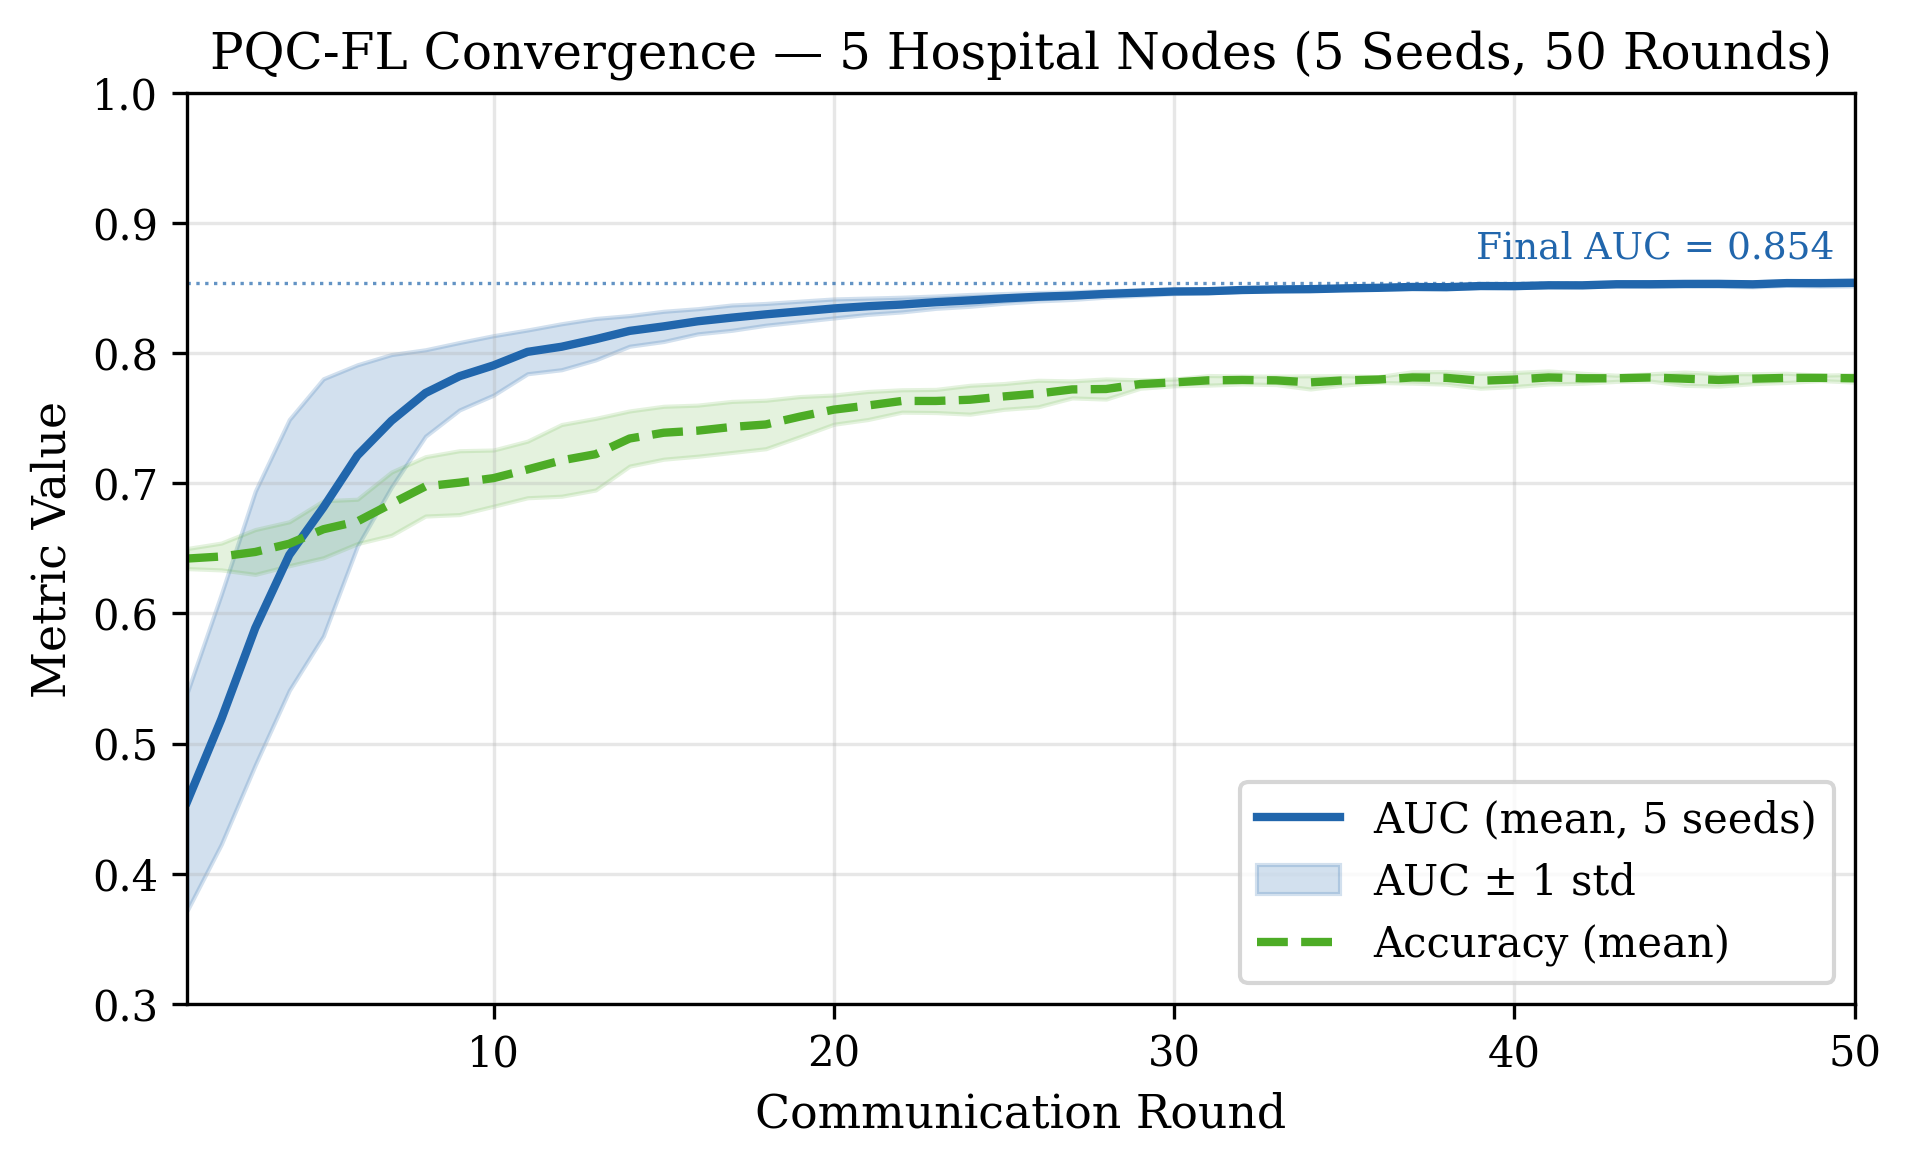
\includegraphics[width=\textwidth]{fig1_convergence.png}
  \caption{FL convergence over 50 rounds across 5 random seeds.
    \textbf{Left:} Heterogeneous federation---5 hospitals spanning diabetes,
    heart disease, and breast cancer datasets (AUC $0.854 \pm 0.002$).
    \textbf{Right:} Homogeneous federation---5 diabetes clinics partitioned
    non-IID by glucose quartile (AUC $0.787 \pm 0.019$).
    Shaded bands show $\pm 1$ standard deviation across seeds.}
  \label{fig:convergence}
\end{figure*}

\begin{table}[t]
  \caption{Final Model Quality (Round 50, 5 Seeds)}
  \label{tab:convergence}
  \centering
  \begin{tabular}{lcc}
    \toprule
    \textbf{Metric} & \textbf{Heterogeneous} & \textbf{Homogeneous (Pima)} \\
    \midrule
    AUC              & $0.854 \pm 0.002$ & $0.787 \pm 0.019$ \\
    Sensitivity      & $0.589 \pm 0.012$ & $0.312 \pm 0.067$ \\
    Specificity      & $0.889 \pm 0.008$ & $0.900 \pm 0.033$ \\
    F1 Score         & $0.660 \pm 0.005$ & $0.412 \pm 0.064$ \\
    Accuracy         & $0.781 \pm 0.003$ & $0.696 \pm 0.023$ \\
    \bottomrule
  \end{tabular}
\end{table}

\subsection{PQC vs.\ Classical Cryptography}

Table~\ref{tab:pqcvscls} compares PQC (ML-KEM-768 + ML-DSA-65 +
AES-256-GCM) against the classical baseline (RSA-4096 + HMAC-SHA256 +
AES-256-GCM) over 30 rounds, 5 nodes.
The two schemes converge to \emph{identical} model quality
(AUC~0.837), confirming that PQC introduces no accuracy degradation.

PQC is \textbf{1.6$\times$ faster} per round (64\,ms vs.\ 101\,ms).
The advantage is driven by decryption: ML-KEM-768 decapsulation takes
1.41\,ms per round, while RSA-4096 decryption takes 33.44\,ms---a
\textbf{24$\times$ speedup}---because RSA's decryption cost scales
with key size while lattice-based KEM decapsulation is $O(n \log n)$
in the polynomial ring dimension.
Fig.~\ref{fig:latency} shows per-round latency traces across all 30 rounds.

\begin{table}[t]
  \caption{PQC vs.\ Classical: 30 Rounds, 5 Nodes}
  \label{tab:pqcvscls}
  \centering
  \begin{tabular}{lrr}
    \toprule
    \textbf{Metric} & \textbf{PQC} & \textbf{Classical} \\
    \midrule
    AUC                      & 0.837 & 0.837 \\
    Avg round time (ms)      & 64    & 101   \\
    Avg enc / node (ms)      & 0.57  & 0.29  \\
    Avg dec / round (ms)     & 1.41  & 33.44 \\
    Total bandwidth (30r)    & 3381\,KB & 2531\,KB \\
    Crypto overhead / round  & 31.1\,KB & 2.8\,KB \\
    \bottomrule
  \end{tabular}
\end{table}

\begin{figure*}[t]
  \centering
  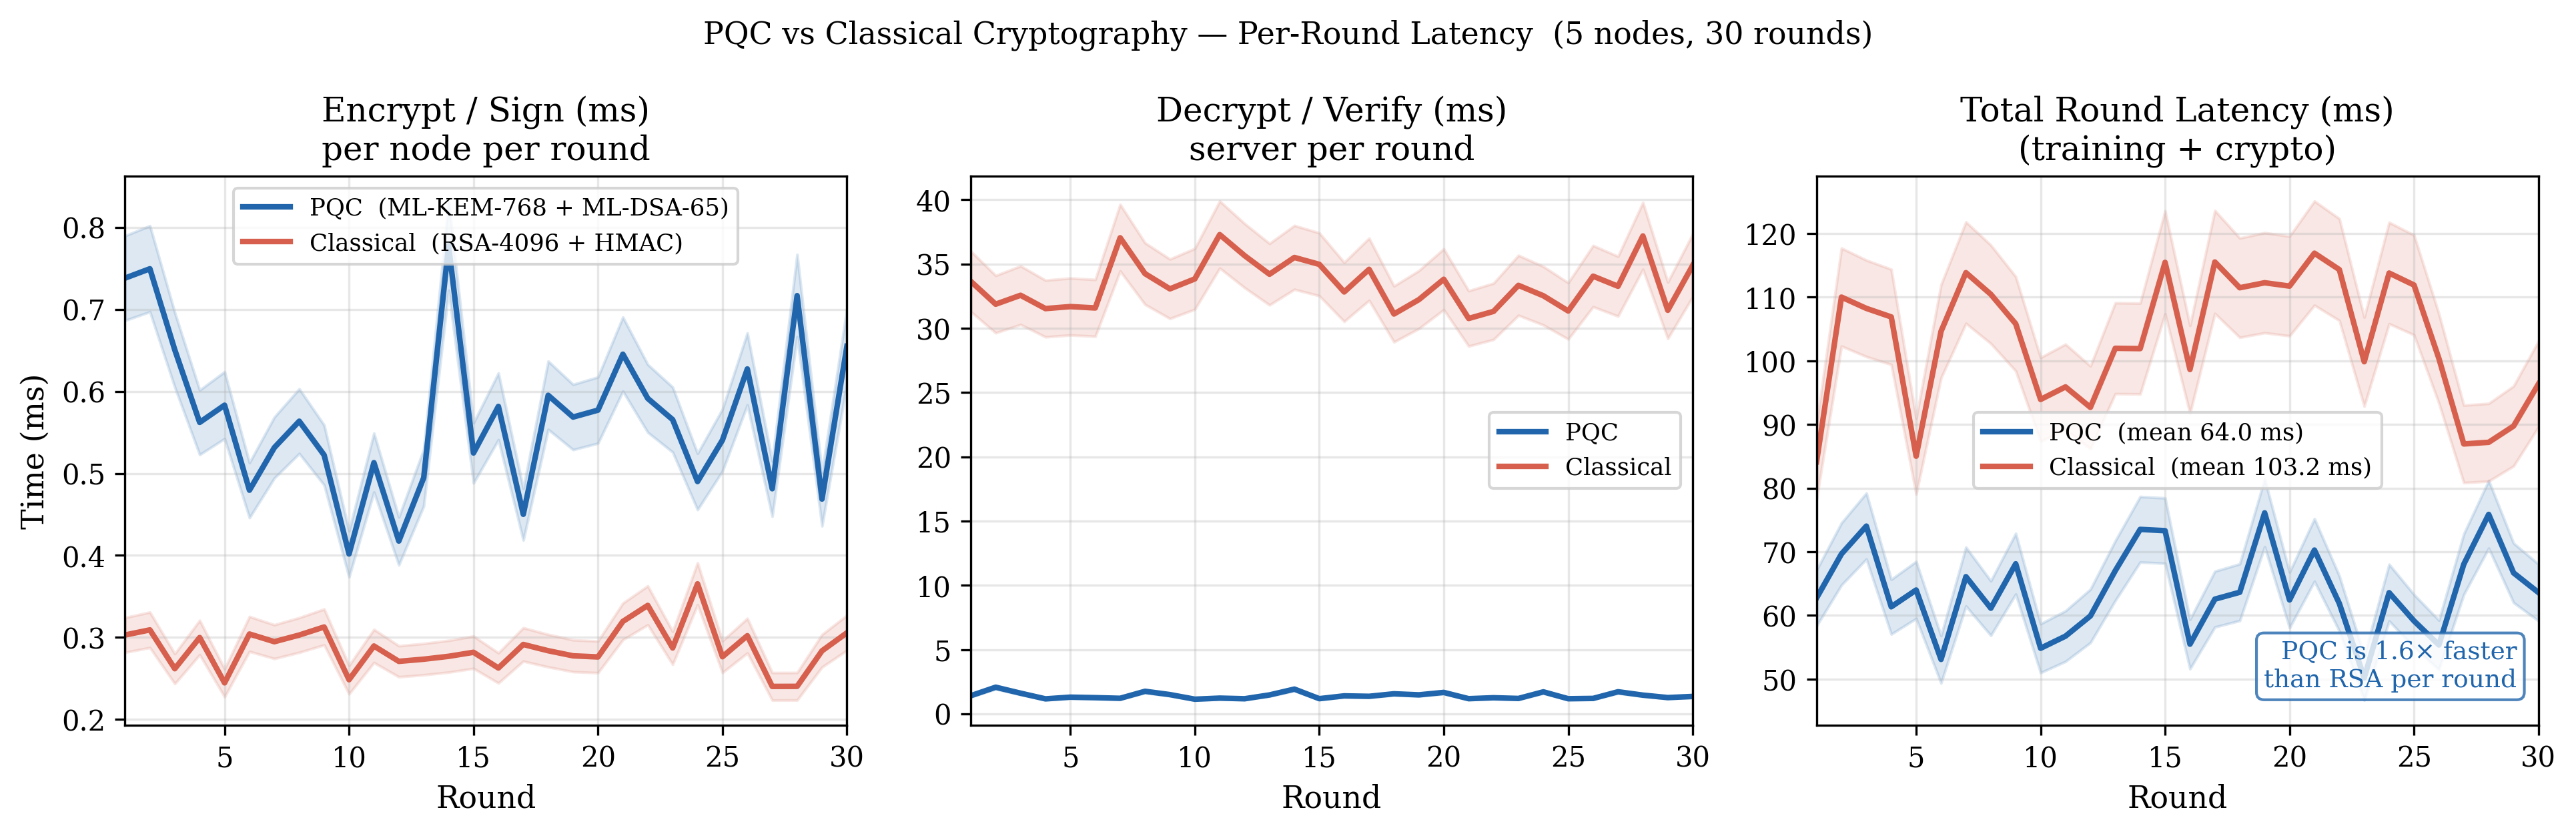
\includegraphics[width=\textwidth]{fig4_latency_breakdown.png}
  \caption{Per-round latency breakdown over 30 rounds (5 nodes).
    \textbf{Left:} Node-side encrypt+sign time per round.
    \textbf{Centre:} Server-side decrypt+verify time per round.
    \textbf{Right:} Total round time (training + cryptography).
    PQC decryption (1.41\,ms) is 24$\times$ faster than RSA-4096 (33.44\,ms),
    yielding a 1.6$\times$ end-to-end speedup (64\,ms vs.\ 101\,ms).}
  \label{fig:latency}
\end{figure*}

\subsection{NIST Security Level Comparison}

Fig.~\ref{fig:seclevels} and Table~\ref{tab:seclevels} benchmark
all three NIST post-quantum security levels on a 12\,KB model-delta
payload (20 iterations each).
Round-trip latency is below 1\,ms at all levels.
Counterintuitively, Level~3 (ML-KEM-768 + ML-DSA-65) is \emph{faster}
than Level~1 in our environment (0.713\,ms vs.\ 0.940\,ms), which we
attribute to CPU cache effects and the specific optimisation profile
of liboqs~0.15.0.
Cryptographic overhead grows monotonically: 4.4\,KB (Level~1),
6.2\,KB (Level~3), 8.6\,KB (Level~5).
For a 12\,KB model delta, even the highest security level adds only
72\% overhead in bytes---a modest cost for quantum-safe guarantees.

\begin{table}[t]
  \caption{NIST Security Level Comparison (12\,KB payload, 20 iter.)}
  \label{tab:seclevels}
  \centering
  \begin{tabular}{lccc}
    \toprule
    \textbf{Metric} & \textbf{Level~1} & \textbf{Level~3} & \textbf{Level~5} \\
    & ML-KEM-512 & ML-KEM-768 & ML-KEM-1024 \\
    & +ML-DSA-44 & +ML-DSA-65 & +ML-DSA-87 \\
    \midrule
    Enc+Sign (ms)       & 0.72 & 0.41 & 0.46 \\
    Dec+Verify (ms)     & 0.22 & 0.31 & 0.31 \\
    Round-trip (ms)     & 0.94 & 0.71 & 0.77 \\
    KEM ciphertext (B)  & 768  & 1088 & 1568 \\
    Signature (B)       & 2420 & 3293 & 4595 \\
    Crypto overhead (KB)& 4.4  & 6.2  & 8.6  \\
    \bottomrule
  \end{tabular}
\end{table}

\begin{figure*}[t]
  \centering
  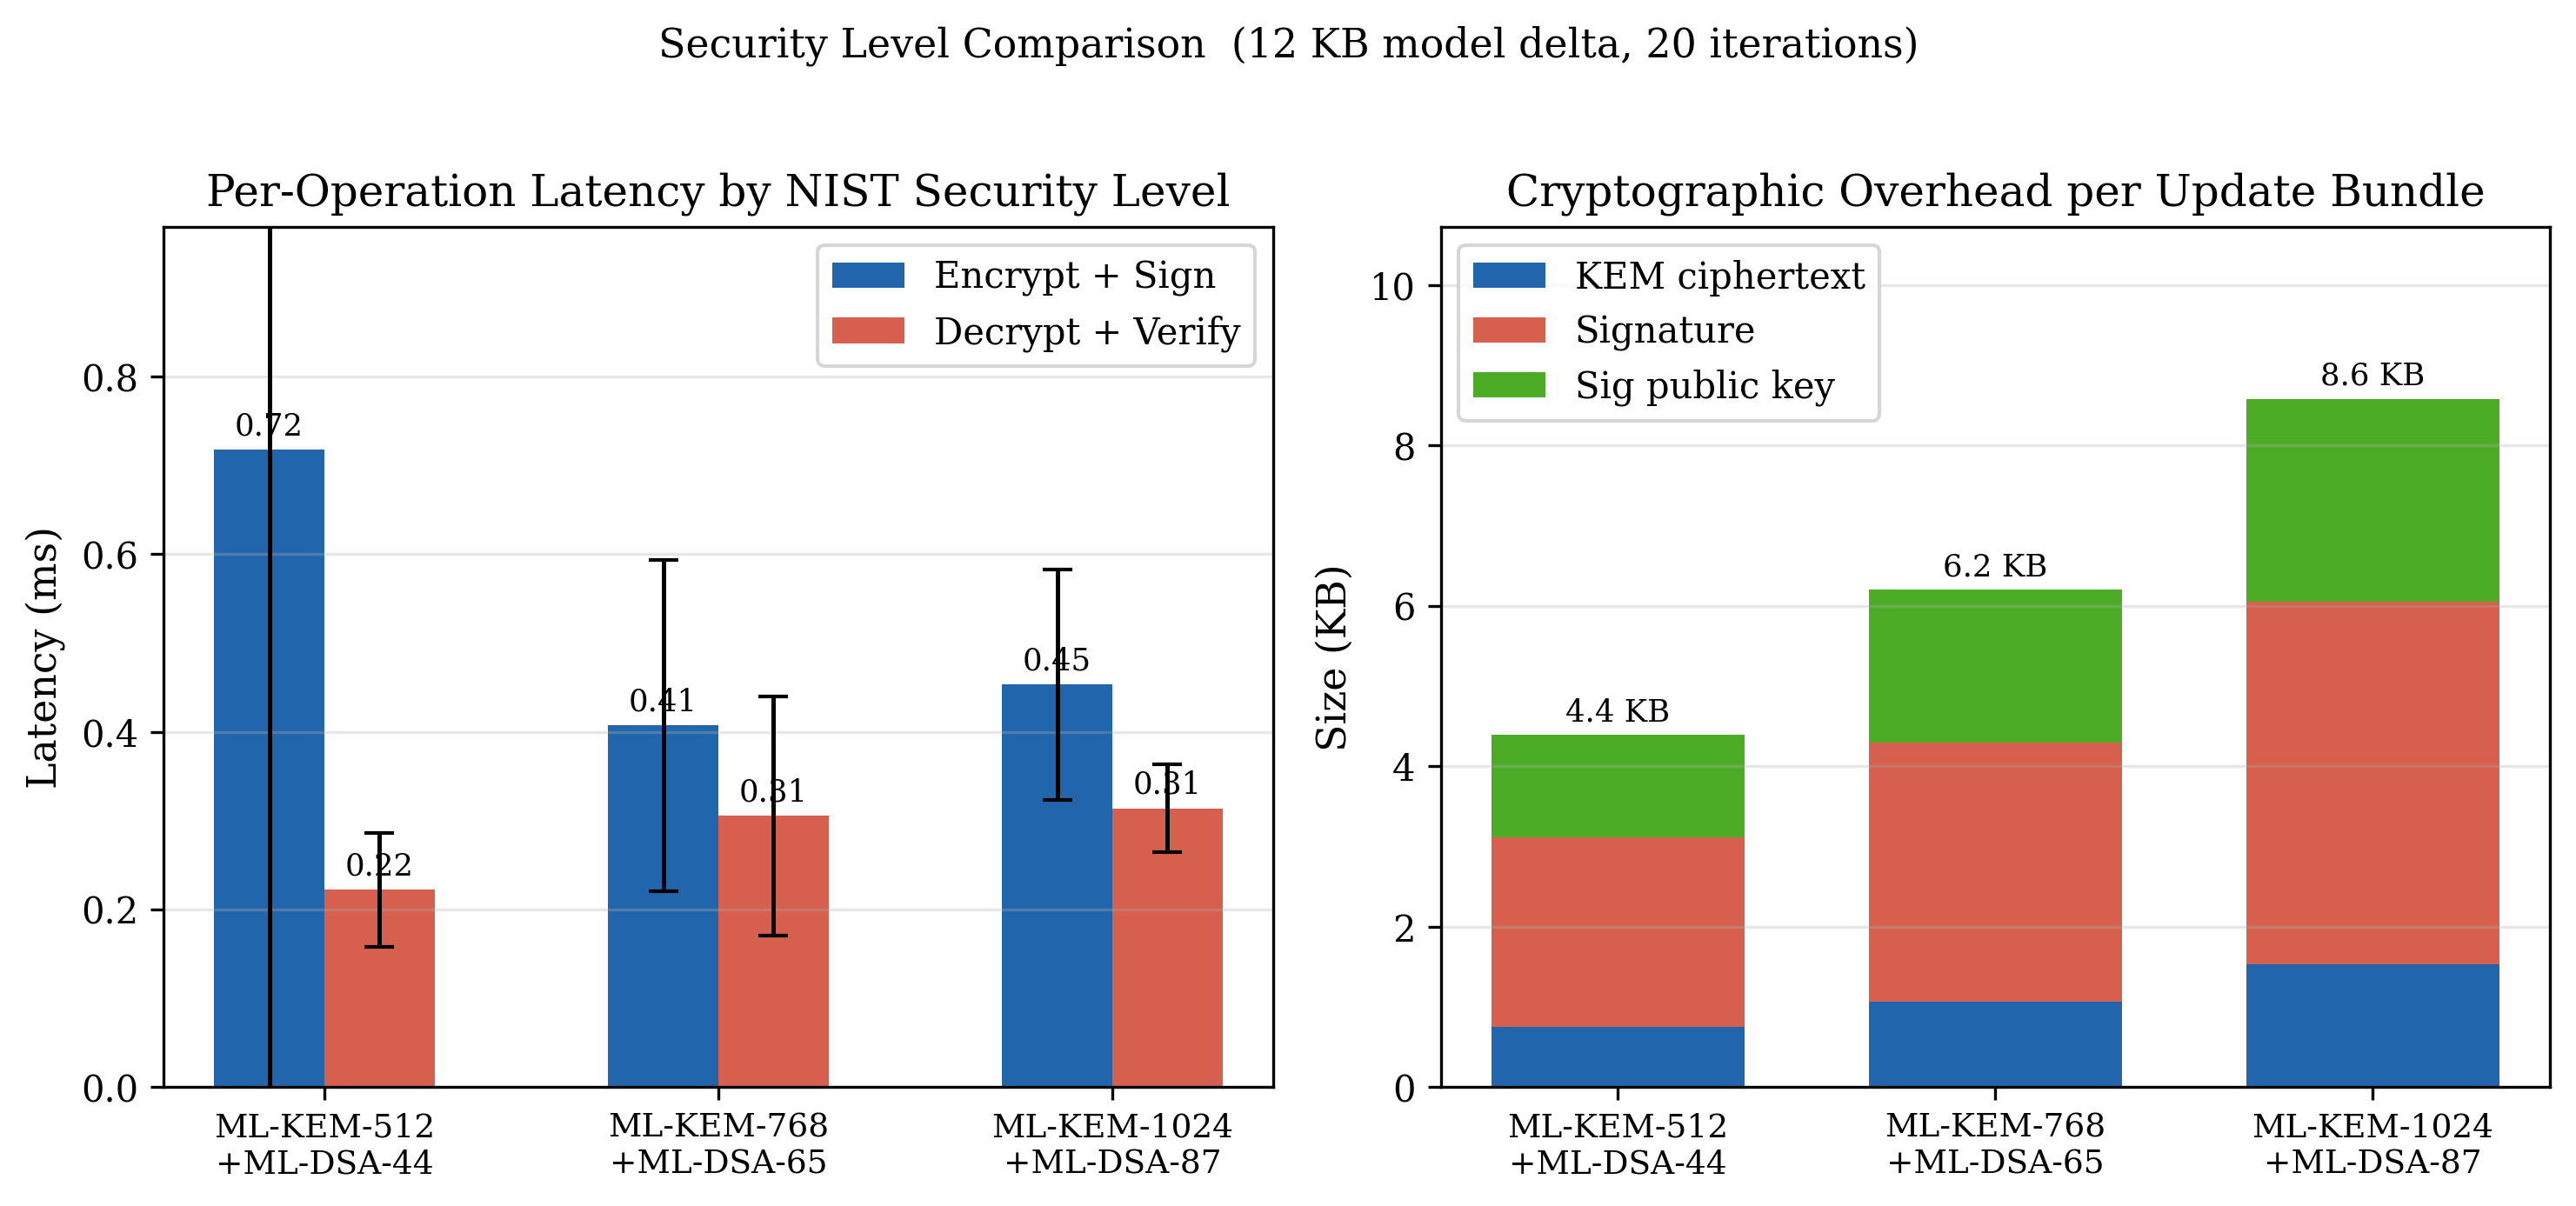
\includegraphics[width=\textwidth]{fig2_security_levels.png}
  \caption{NIST post-quantum security level comparison on a 12\,KB model-delta payload
    (20 iterations each).
    \textbf{Left:} Per-operation latency (mean $\pm$ std).
    All levels complete encrypt+sign and decrypt+verify in under 0.8\,ms.
    \textbf{Right:} Cryptographic overhead per update bundle, decomposed
    into KEM ciphertext, signature, and signing public key.
    Overhead grows from 4.4\,KB (Level~1) to 8.6\,KB (Level~5).}
  \label{fig:seclevels}
\end{figure*}

\subsection{Byzantine Attack and Defence}

Fig.~\ref{fig:byzantine} shows the two-part Byzantine evaluation
over 20 rounds with node~4 as the rogue node.

\textbf{Part A: Tampered Signature Attack.}
The rogue node flips the first 32 bytes of its ML-DSA signature
before transmission.
ML-DSA verification rejects the bundle in \textbf{100\% of rounds
(20/20)}.
The global model trains on the remaining four honest nodes and
converges more slowly than the clean baseline, reflecting the lost
data contribution from one hospital shard---but \emph{no adversarial
gradient ever enters the global model}.

\textbf{Part B: Gradient Poisoning Attack.}
The rogue node sends a correctly signed but 50$\times$-scaled gradient
delta.
Without the norm filter, the poisoned model reaches AUC~0.789,
which is 7.6\% below the clean baseline (0.854).
With the gradient-norm filter ($3\times$ median threshold), the rogue
node is rejected in \textbf{100\% of rounds (20/20)}.
These results demonstrate that ML-DSA authentication provides a
cryptographic first line of defence, while the statistical norm filter
forms an effective second line.

\begin{figure*}[t]
  \centering
  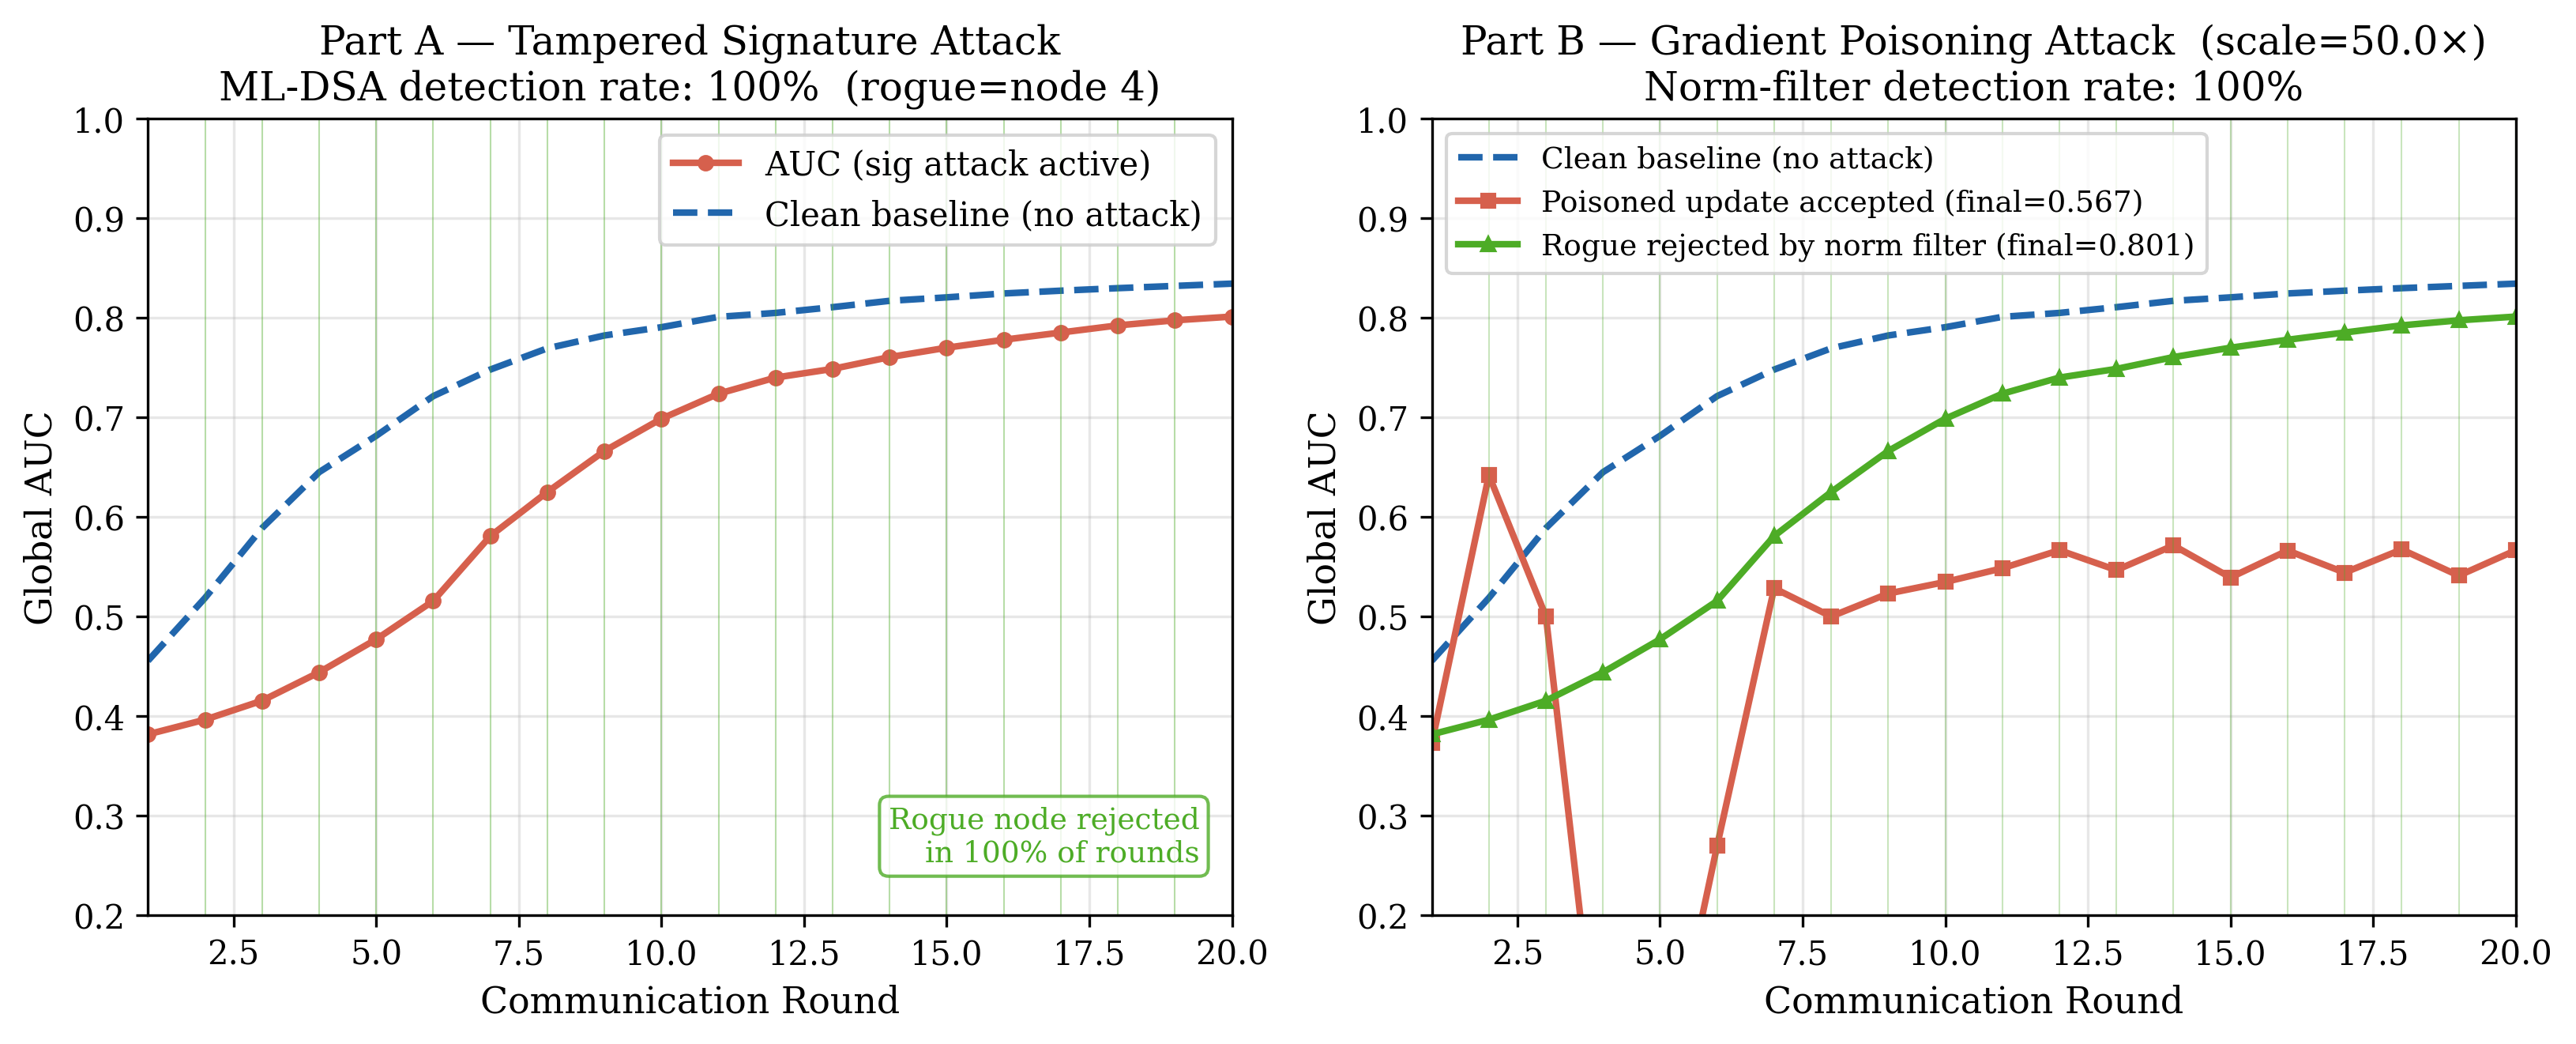
\includegraphics[width=\textwidth]{fig3_byzantine.png}
  \caption{Byzantine attack evaluation over 20 rounds (node~4 as rogue, seed~42).
    \textbf{Left (Part~A):} Tampered-signature attack.
    ML-DSA rejects the rogue node in 100\% of rounds; the global model
    trains on the four honest hospitals only.
    \textbf{Right (Part~B):} Gradient-poisoning attack (50$\times$ scale).
    Without defence, AUC drops to 0.789 (7.6\% below clean baseline).
    With gradient-norm filter, the rogue is rejected in 100\% of rounds.
    Vertical lines mark rounds where the rogue was detected and rejected.}
  \label{fig:byzantine}
\end{figure*}

\subsection{Differential Privacy Tradeoff}

Fig.~\ref{fig:dp} and Table~\ref{tab:dp} show the privacy-utility
tradeoff across six epsilon values (30 rounds, seed~42, clip $S=0.1$,
$\delta=10^{-5}$, $\text{lr}=0.01$).

At $\varepsilon = \infty$ (no DP), the model reaches AUC~0.845.
At $\varepsilon = 50$, the penalty is only $-1.3\%$ (AUC~0.834).
At $\varepsilon = 10$, the penalty is $-4.4\%$ (AUC~0.808).
Tighter budgets ($\varepsilon \le 5$) cause severe degradation:
AUC~0.741 at $\varepsilon=5$ and near-random performance at
$\varepsilon \le 1$.

This steep degradation at small $\varepsilon$ is a known
characteristic of DP in small-model FL~\cite{geyer2017}: with only
1531 parameters, the Gaussian noise ($\sigma = 0.484$ at
$\varepsilon=1$) overwhelms the gradient signal ($\|\Delta\|_2
\approx 0.07$).
The result provides a practical recommendation: \textbf{for this model
class, $\varepsilon \ge 10$ provides meaningful privacy at acceptable
utility cost}.

\begin{figure*}[t]
  \centering
  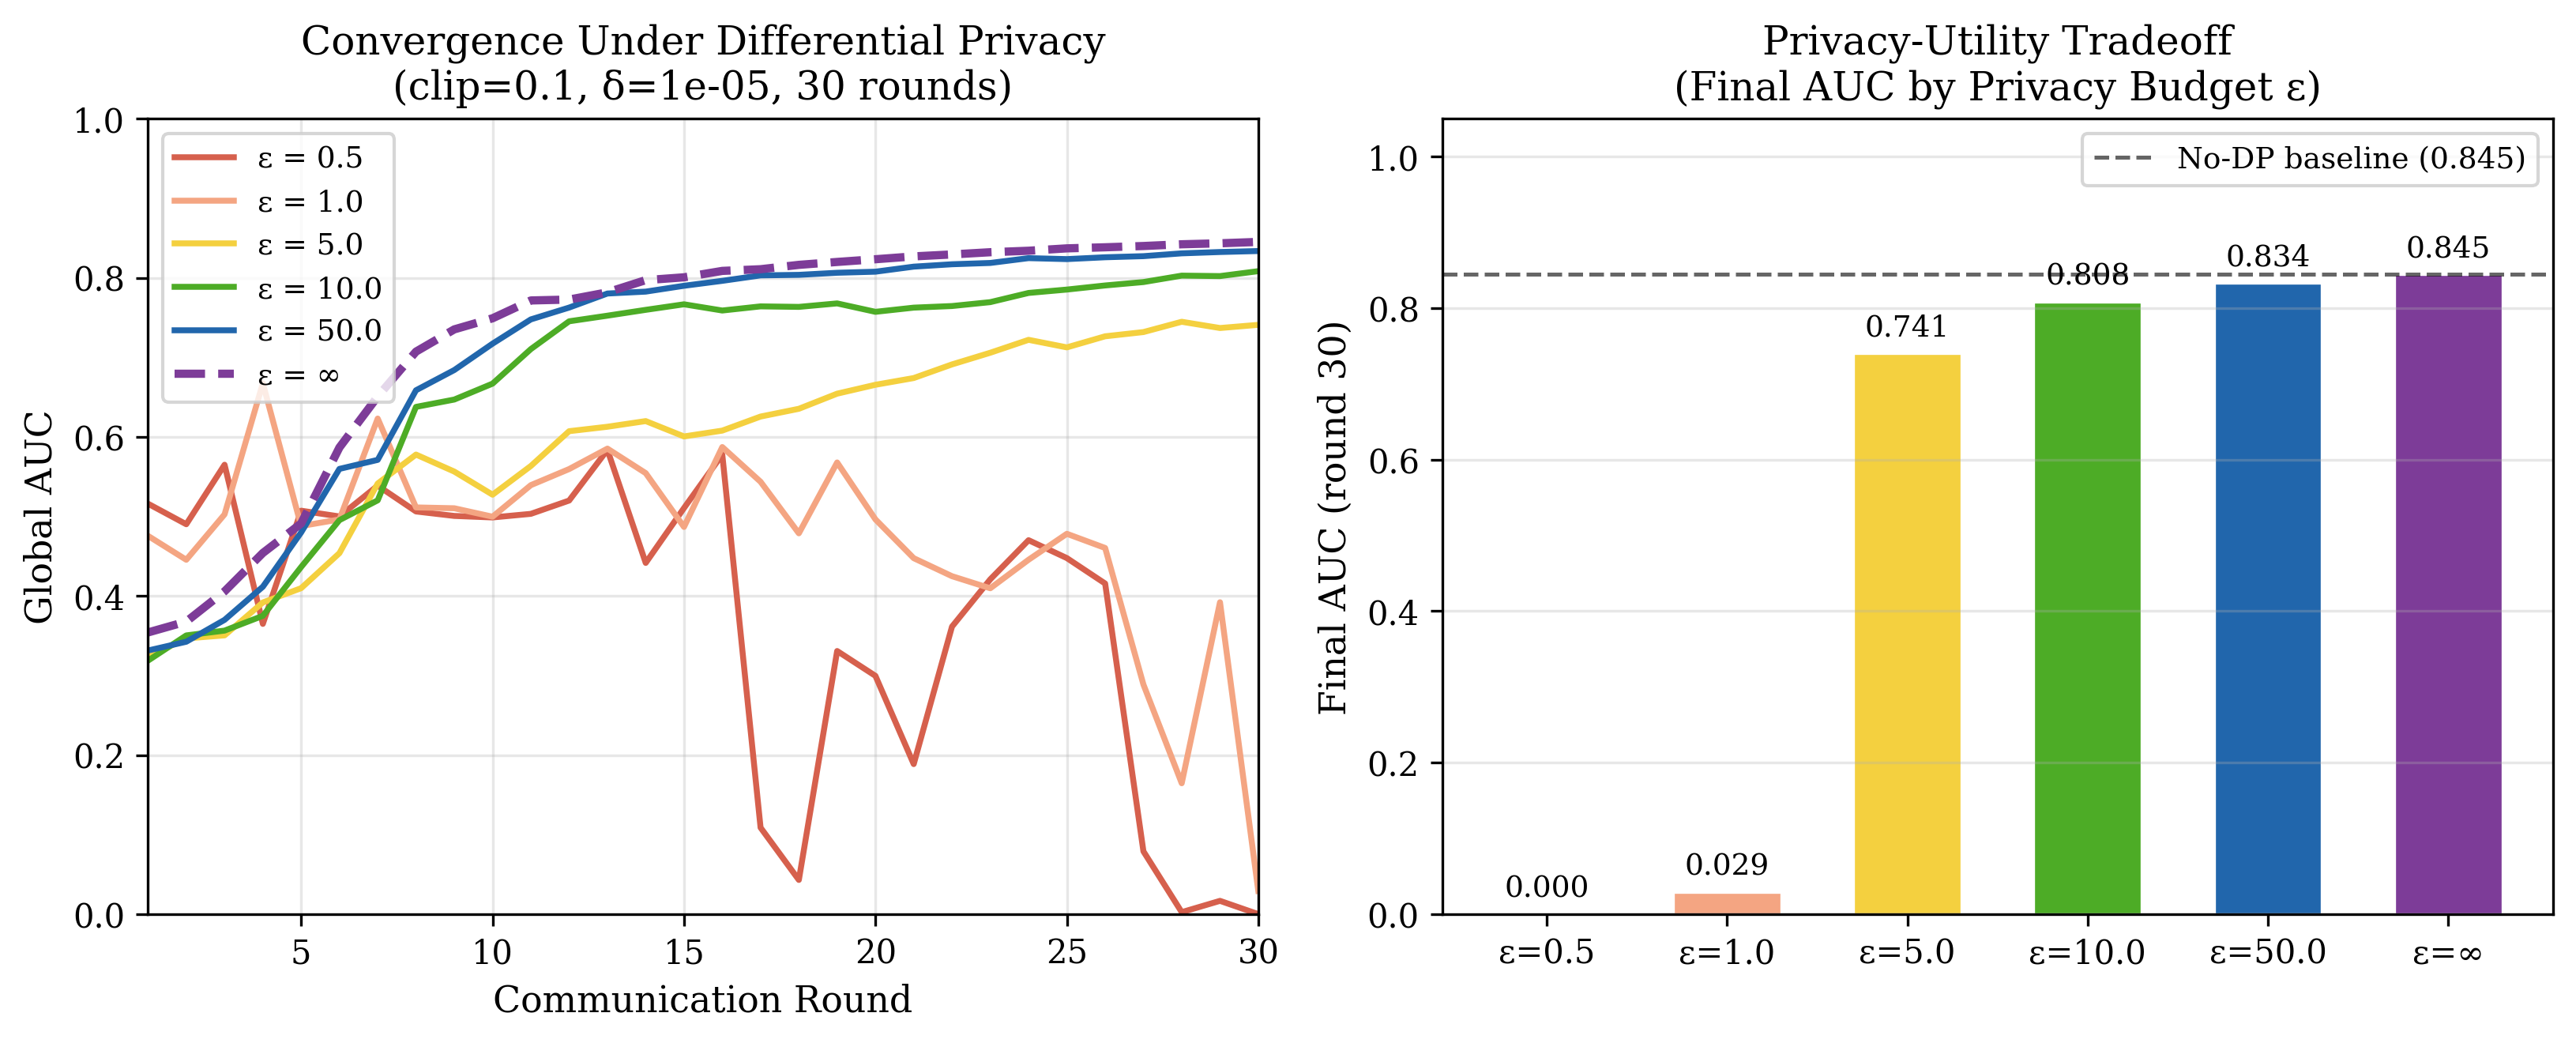
\includegraphics[width=\textwidth]{fig5_dp_tradeoff.png}
  \caption{Differential privacy privacy-utility tradeoff
    (30 rounds, seed~42, clip $S=0.1$, $\delta=10^{-5}$).
    \textbf{Left:} Convergence curves for each $\varepsilon$ value.
    $\varepsilon=50$ (blue) nearly matches the no-DP baseline (purple dashed).
    \textbf{Right:} Final AUC at round~30 vs.\ privacy budget.
    The dashed line marks the no-DP baseline (AUC~0.845).
    At $\varepsilon=10$, the AUC penalty is only $-4.4\%$.
    At $\varepsilon \le 1$, the noise overwhelms the gradient signal.}
  \label{fig:dp}
\end{figure*}

\begin{table}[t]
  \caption{Differential Privacy: Final AUC (Round 30) vs.\ $\varepsilon$}
  \label{tab:dp}
  \centering
  \begin{tabular}{ccc}
    \toprule
    $\varepsilon$ & $\sigma$ & \textbf{AUC (Round 30)} \\
    \midrule
    0.5   & 0.969 & 0.000 \\
    1.0   & 0.484 & 0.029 \\
    5.0   & 0.097 & 0.741 \\
    10.0  & 0.048 & 0.808 \\
    50.0  & 0.010 & 0.834 \\
    $\infty$ & 0   & 0.845 \\
    \bottomrule
  \end{tabular}
\end{table}

\subsection{Communication Overhead}

Fig.~\ref{fig:overhead} decomposes per-round bandwidth into model
payload and cryptographic overhead.
Each round, all five nodes transmit their update bundles (total 112.7\,KB
for PQC, 84.4\,KB for classical).
The model payload is approximately 81.6\,KB (identical for both
schemes).
PQC cryptographic overhead averages 31.1\,KB per round (27.6\% of
total), comprising ML-KEM ciphertexts (1088\,B $\times$ 5 = 5.3\,KB),
ML-DSA-65 signatures (3293\,B $\times$ 5 = 16.1\,KB), and signing
public keys (1952\,B $\times$ 5 = 9.5\,KB).
Classical overhead is only 2.8\,KB, but pays a 24$\times$ latency
penalty on decryption.
Over a 30-round training run, PQC consumes 850\,KB more bandwidth
than the classical baseline---at 1\,Mbps (a typical hospital VPN),
this represents an additional 6.8\,seconds per complete run, which
is negligible relative to the quantum-safety guarantee obtained.

\begin{figure*}[t]
  \centering
  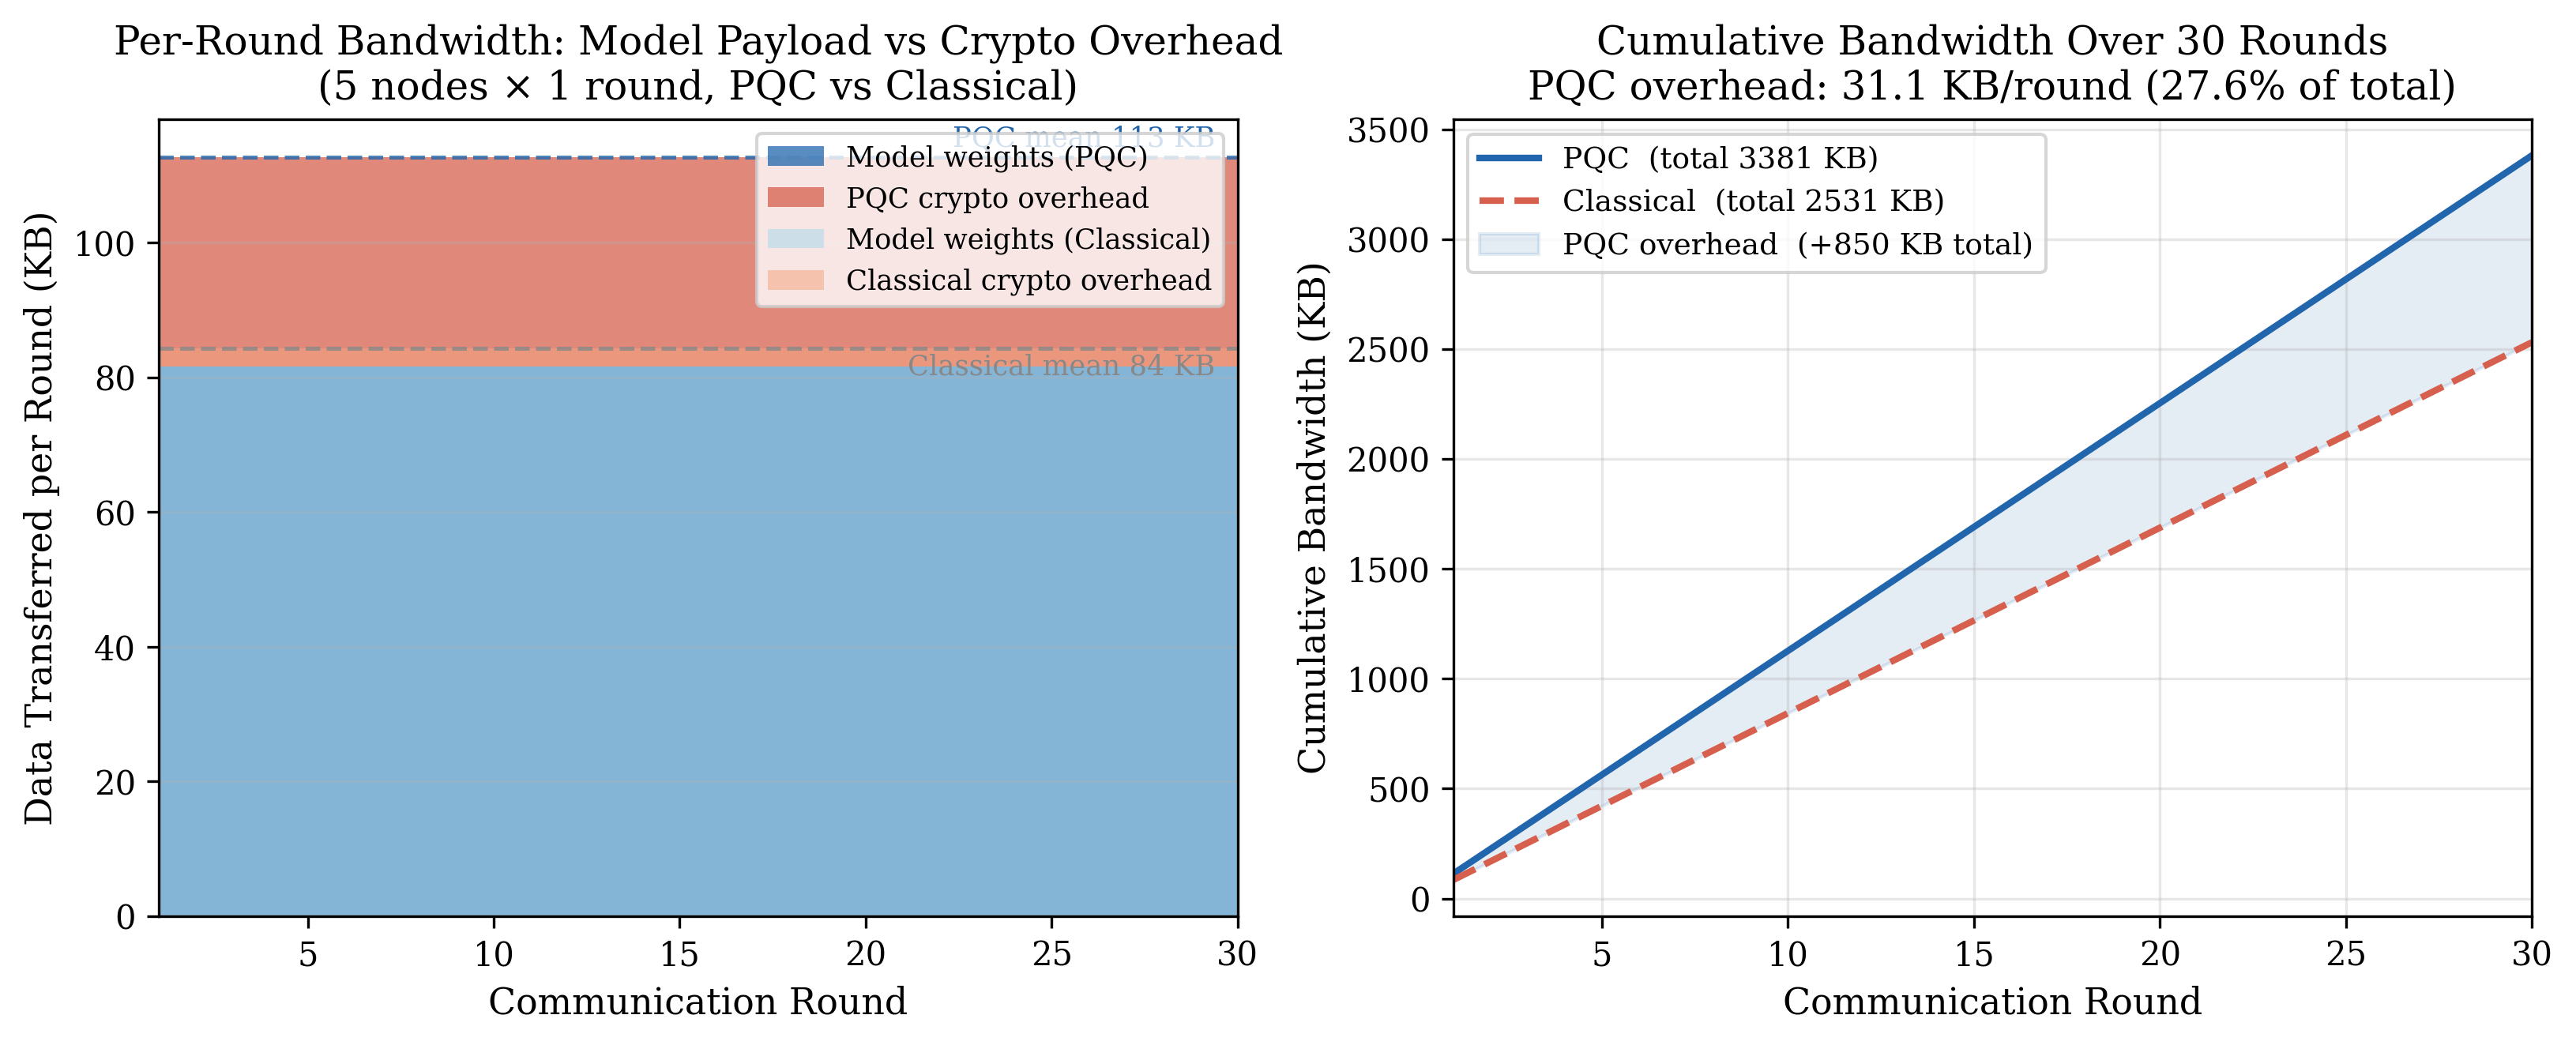
\includegraphics[width=\textwidth]{fig6_comm_overhead.png}
  \caption{Communication overhead analysis over 30 rounds (5 nodes).
    \textbf{Left:} Per-round bandwidth decomposed into model weights
    (payload) and cryptographic overhead.
    PQC adds 31.1\,KB/round (27.6\% of total); Classical adds 2.8\,KB/round.
    \textbf{Right:} Cumulative bandwidth.
    PQC totals 3381\,KB vs.\ 2531\,KB for Classical---an 850\,KB difference
    over 30 rounds, equivalent to 6.8\,s on a 1\,Mbps hospital VPN.}
  \label{fig:overhead}
\end{figure*}

%==================================================================
\section{Discussion}
\label{sec:discussion}

\subsection{Why PQC Is Faster Despite More Bytes}

The counterintuitive finding---PQC is simultaneously \emph{larger}
and \emph{faster} than RSA---arises because latency and bandwidth are
decoupled in our setting.
RSA-4096 decryption is computationally expensive ($O(k^3)$ in key
bits), dominating the 33.44\,ms classical decryption cost.
ML-KEM-768 decapsulation is purely ring arithmetic ($O(n \log n)$),
finishing in under 0.3\,ms.
The additional KEM ciphertext and signature bytes cost bandwidth but
not computation.

\subsection{Heterogeneous vs.\ Homogeneous Federation}

The 8.7\% AUC gap between heterogeneous (0.854) and homogeneous
Pima-only (0.787) federation may seem surprising.
The key factor is the severity of label skew: the glucose-quartile
non-IID split produces a 9$\times$ label ratio across nodes (8.1\%
to 73.2\% positive), which is among the most extreme distributions
studied in FL literature~\cite{zhao2018}.
Heterogeneous federation inadvertently mitigates this by
aggregating across disease domains with more balanced class ratios.
This suggests that, where privacy regulations permit, cross-institution
data sharing across related disease domains may improve FL convergence
more than within-disease data accumulation.

\subsection{Limitations}

Several limitations of this work should be acknowledged.
First, our model is intentionally small (1531 parameters) for
transparency and reproducibility; larger models would likely
accommodate tighter DP budgets.
Second, experiments run on a single CPU without hardware acceleration;
real hospital deployments may use dedicated HSMs for key management
and hardware-accelerated lattice arithmetic.
Third, the Byzantine experiments consider a single rogue node (1~of~5);
future work should characterise the detection threshold as the fraction
of Byzantine nodes grows.
Fourth, while we simulate non-IID data heterogeneity, we do not
model network latency or asynchronous updates.

%==================================================================
\section{Conclusion}
\label{sec:conclusion}

We presented PQC-FL-Health, a federated learning framework for
healthcare that provides three complementary privacy guarantees:
quantum-safe confidentiality (ML-KEM-768), authenticated gradient
integrity (ML-DSA-65), and aggregator-side patient privacy
(Gaussian DP).
On a five-hospital heterogeneous federation spanning three disease
domains, the system achieves AUC $0.854 \pm 0.002$ over 50 rounds
and 5 seeds.
PQC operations complete in under 1\,ms at all NIST security levels
and are 1.6$\times$ faster end-to-end than RSA-4096, despite
producing 11$\times$ more cryptographic bytes per update.
An ML-DSA-based Byzantine filter achieves 100\% detection on both
tampered-signature and gradient-poisoning attacks.
The DP layer quantifies an explicit privacy-utility tradeoff:
$\varepsilon \ge 10$ costs under 5\% AUC for this model class.
We further demonstrate system generalisability on a Pima-only
homogeneous federation, characterising the non-IID penalty under
extreme glucose-quartile partitioning.

As quantum hardware continues to mature, we argue that federated
healthcare systems should adopt PQC not as a future upgrade but as
a present design requirement.
PQC-FL-Health demonstrates that quantum-safe FL is achievable
today with no accuracy cost and a latency advantage over the
classical baseline it replaces.

%==================================================================
\section*{Acknowledgment}
The authors thank the open-source contributors to the Open Quantum
Safe project~\cite{oqs} for providing the liboqs library used in
all experiments.

%==================================================================
\begin{thebibliography}{00}

\bibitem{mcmahan2017}
H.~B. McMahan, E.~Moore, D.~Ramage, S.~Hampson, and B.~A.~y~Arcas,
``Communication-Efficient Learning of Deep Networks from Decentralized
Data,'' in \emph{Proc. AISTATS}, 2017.

\bibitem{shor1994}
P.~W. Shor, ``Algorithms for quantum computation: discrete logarithms
and factoring,'' in \emph{Proc. 35th Annual Symposium on Foundations
of Computer Science}, 1994.

\bibitem{nistfips203}
National Institute of Standards and Technology,
``Module-Lattice-Based Key-Encapsulation Mechanism Standard (FIPS 203),''
2024.

\bibitem{nistfips204}
National Institute of Standards and Technology,
``Module-Lattice-Based Digital Signature Standard (FIPS 204),''
2024.

\bibitem{blanchard2017}
P.~Blanchard, E.~M.~El Mhamdi, R.~Guerraoui, and J.~Stainer,
``Machine Learning with Adversaries: Byzantine Tolerant Gradient
Descent,'' in \emph{Proc. NeurIPS}, 2017.

\bibitem{dwork2006}
C.~Dwork, F.~McSherry, K.~Nissim, and A.~Smith,
``Calibrating Noise to Sensitivity in Private Data Analysis,''
in \emph{Proc. TCC}, 2006.

\bibitem{abadi2016}
M.~Abadi \emph{et~al.}, ``Deep Learning with Differential Privacy,''
in \emph{Proc. CCS}, 2016.

\bibitem{geyer2017}
R.~C. Geyer, T.~Klein, and M.~Nabi,
``Differentially Private Federated Learning: A Client Level
Perspective,'' \emph{arXiv:1712.07557}, 2017.

\bibitem{fang2020}
M.~Fang, X.~Cao, J.~Jia, and N.~Gong,
``Local Model Poisoning Attacks to Byzantine-Robust Federated
Learning,'' in \emph{Proc. USENIX Security}, 2020.

\bibitem{geiping2020}
J.~Geiping, H.~Bauermeister, H.~Dr{\"o}ge, and M.~Moeller,
``Inverting Gradients --- How Easy Is It to Break Privacy in
Federated Learning?'' in \emph{Proc. NeurIPS}, 2020.

\bibitem{li2020federated}
T.~Li, A.~K. Sahu, A.~Talwalkar, and V.~Smith,
``Federated Learning: Challenges, Methods, and Future Directions,''
\emph{IEEE Signal Processing Magazine}, vol.~37, no.~3, 2020.

\bibitem{rieke2020}
N.~Rieke \emph{et~al.},
``The future of digital health with federated learning,''
\emph{npj Digital Medicine}, vol.~3, no.~1, 2020.

\bibitem{zhao2018}
Y.~Zhao, M.~Li, L.~Lai, N.~Suda, D.~Civin, and V.~Chandra,
``Federated Learning with Non-IID Data,''
\emph{arXiv:1806.00582}, 2018.

\bibitem{nguyen2021}
D.~C. Nguyen \emph{et~al.},
``Federated Learning for Internet of Things: A Comprehensive Survey,''
\emph{IEEE Commun. Surveys Tuts.}, vol.~23, no.~3, 2021.

\bibitem{oqs}
D.~Stebila and M.~Mosca,
``Post-Quantum Key Exchange for the Internet and the Open Quantum Safe
Project,'' in \emph{Proc. SAC}, 2016.

\bibitem{smith1988}
J.~W. Smith \emph{et~al.},
``Using the ADAP Learning Algorithm to Forecast the Onset of Diabetes
Mellitus,'' in \emph{Proc. SCAMC}, 1988.

\bibitem{detrano1989}
R.~Detrano \emph{et~al.},
``International Application of a New Probability Algorithm for the
Diagnosis of Coronary Artery Disease,''
\emph{American Journal of Cardiology}, vol.~64, 1989.

\bibitem{street1993}
W.~N. Street, W.~H. Wolberg, and O.~L. Mangasarian,
``Nuclear Feature Extraction for Breast Tumor Diagnosis,''
in \emph{SPIE Proc. Electronic Imaging}, vol.~1905, 1993.

\end{thebibliography}

\end{document}
